\documentclass[tikz]{standalone}

\usepackage{tikz}
\usetikzlibrary{trees}
\usetikzlibrary{shapes}
\usetikzlibrary{positioning}
\usetikzlibrary{arrows.meta}

\tikzset{
    mynode/.style = {circle, ultra thick, draw=black, align=center,fill=yellow!30,font=\ttfamily\bfseries\Large,text=black},
    mynoder/.style = {circle, ultra thick, draw=black, align=center,fill=red!30,font=\ttfamily\bfseries\Large,text=black},
    mynodeb/.style = {circle, ultra thick, draw=black, align=center,fill=blue!30,font=\ttfamily\bfseries\Large,text=black},
    mynodeg/.style = {circle, ultra thick, draw=gray, align=center,fill=gray!05,font=\ttfamily\bfseries\Large,text=gray!20},
    mynodegr/.style = {circle, ultra thick, draw=gray, align=center,fill=gray!05,font=\ttfamily\bfseries\Large,text=red},
    edgen/.style = {-,ultra thick,black},
    edger/.style = {-,ultra thick,red},
    edgeb/.style = {-,ultra thick,blue},
    edgeg/.style = {-,ultra thick,gray},
    edgegd/.style = {-,ultra thick,brown,dashed}, % back
    edgevd/.style = {-,ultra thick,violet,dotted}, % forward
    edgexd/.style = {-,ultra thick,blue,densely dotted}, % traversal
    every picture/.style={/utils/exec={\ttfamily\bfseries}},
    every picture/.style={font issue=\ttfamily\bfseries},
    font issue/.style={execute at begin picture={#1\selectfont}}
}

\begin{document}



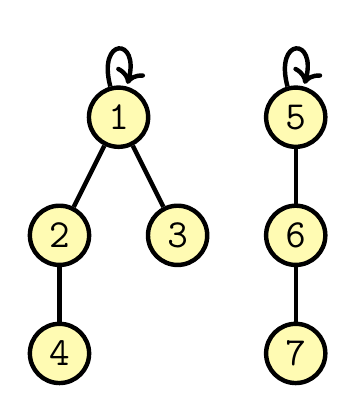
\begin{tikzpicture}[thick,font=\ttfamily\bfseries]
\node[mynode] at (0, 0) (a4) {4};
\node[mynode] at (0, 1.5) (a2) {2};
\node[mynode] at (1.5, 1.5) (a3) {3};
\node[mynode] at (0.75, 3) (a1) {1};
\node[mynode] at (3, 3) (b5) {5};
\node[mynode] at (3, 1.5) (b6) {6};
\node[mynode] at (3, 0) (b7) {7};
%
\draw[edgen] (a4) edge node {} (a2);
\draw[edgen] (a2) edge node {} (a1);
\draw[edgen] (a3) edge node {} (a1);
\draw[edgen] (a1) edge[loop above,->] node {} (a1);
\draw[edgen] (b7) edge node {} (b6);
\draw[edgen] (b6) edge node {} (b5);
\draw[edgen,->] (b5) edge[loop above] node[->] {} (b5);

\end{tikzpicture}


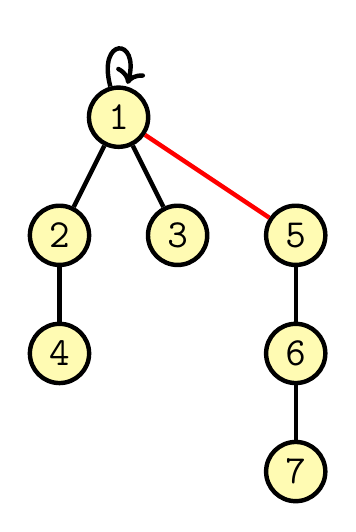
\begin{tikzpicture}[thick,font=\ttfamily\bfseries]
\node[mynode] at (0, 0) (a4) {4};
\node[mynode] at (0, 1.5) (a2) {2};
\node[mynode] at (1.5, 1.5) (a3) {3};
\node[mynode] at (0.75, 3) (a1) {1};
\node[mynode] at (3, 1.5) (b5) {5};
\node[mynode] at (3, 0) (b6) {6};
\node[mynode] at (3, -1.5) (b7) {7};
%
\draw[edgen] (a4) edge node {} (a2);
\draw[edgen] (a2) edge node {} (a1);
\draw[edgen] (a3) edge node {} (a1);
\draw[edgen] (a1) edge[loop above,->] node {} (a1);
\draw[edgen] (b7) edge node {} (b6);
\draw[edgen] (b6) edge node {} (b5);
\draw[edger] (b5) edge node {} (a1);

\end{tikzpicture}

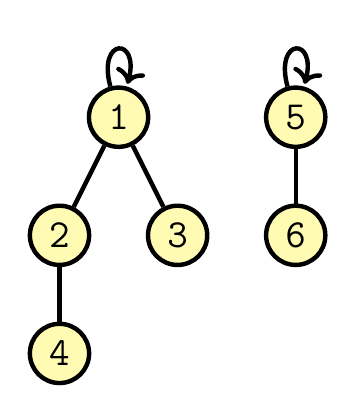
\begin{tikzpicture}[thick,font=\ttfamily\bfseries]
\node[mynode] at (0, 0) (a4) {4};
\node[mynode] at (0, 1.5) (a2) {2};
\node[mynode] at (1.5, 1.5) (a3) {3};
\node[mynode] at (0.75, 3) (a1) {1};
\node[mynode] at (3, 3) (b5) {5};
\node[mynode] at (3, 1.5) (b6) {6};
%
\draw[edgen] (a4) edge node {} (a2);
\draw[edgen] (a2) edge node {} (a1);
\draw[edgen] (a3) edge node {} (a1);
\draw[edgen] (a1) edge[loop above,->] node {} (a1);
\draw[edgen] (b6) edge node {} (b5);
\draw[edgen,->] (b5) edge[loop above] node[->] {} (b5);

\end{tikzpicture}

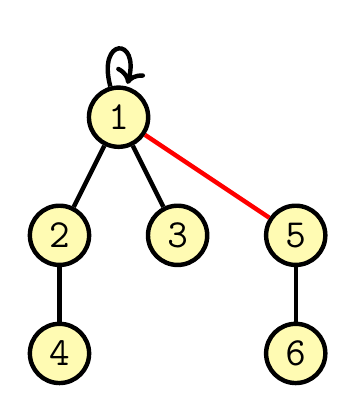
\begin{tikzpicture}[thick,font=\ttfamily\bfseries]
\node[mynode] at (0, 0) (a4) {4};
\node[mynode] at (0, 1.5) (a2) {2};
\node[mynode] at (1.5, 1.5) (a3) {3};
\node[mynode] at (0.75, 3) (a1) {1};
\node[mynode] at (3, 1.5) (b5) {5};
\node[mynode] at (3, 0) (b6) {6};
%
\draw[edgen] (a4) edge node {} (a2);
\draw[edgen] (a2) edge node {} (a1);
\draw[edgen] (a3) edge node {} (a1);
\draw[edgen] (a1) edge[loop above,->] node {} (a1);
\draw[edgen] (b6) edge node {} (b5);
\draw[edger] (b5) edge node {} (a1);

\end{tikzpicture}


\end{document}
